% Copyright 2004 by Till Tantau <tantau@users.sourceforge.net>.
%
% In principle, this file can be redistributed and/or modified under
% the terms of the GNU Public License, version 2.
%
% However, this file is supposed to be a template to be modified
% for your own needs. For this reason, if you use this file as a
% template and not specifically distribute it as part of a another
% package/program, I grant the extra permission to freely copy and
% modify this file as you see fit and even to delete this copyright
% notice. 

\documentclass[xcolor=dvipsnames]{beamer}
\usepackage{wrapfig}
\usepackage[utf8]{inputenc}
\usepackage{physics}
%\usepackage{wrapfig}
\usepackage{cutwin}

%\usepackage[dvipsnames]{xcolor}
% There are many different themes available for Beamer. A comprehensive
% list with examples is given here:
% http://deic.uab.es/~iblanes/beamer_gallery/index_by_theme.html
% You can uncomment the themes below if you would like to use a different
% one:
%\usetheme{AnnArbor}
%\usetheme{Antibes}
%\usetheme{Bergen}
%\usetheme{Berkeley}
%\usetheme{Berlin}
%\usetheme{Boadilla}
%\usetheme{boxes}
%\usetheme{CambridgeUS}
%\usetheme{Copenhagen}
%\usetheme{Darmstadt}
%\usetheme{default}
%\usetheme{Frankfurt}
%\usetheme{Goettingen}
%\usetheme{Hannover}
%\usetheme{Ilmenau}
%\usetheme{JuanLesPins}
%\usetheme{Luebeck}
%\usetheme{Madrid}
\mode<presentation>
 {
 \usetheme{Berlin}
 \setbeamercolor{frametitle}{fg=YellowOrange,bg=YellowOrange!20}
 \setbeamercolor{section in head/foot}{bg=YellowOrange}
 \setbeamercolor{author in head/foot}{bg=YellowOrange}
 \setbeamercolor{date in head/foot}{fg=YellowOrange}
 \usecolortheme[named=Black]{structure}
 \setbeamerfont{footnote}{size=\footnotesize}
 }

%\usetheme{Marburg}
%\usetheme{Montpellier}
%\usetheme{PaloAlto}
%\usetheme{Pittsburgh}
%\usetheme{Rochester}
%\usetheme{Singapore}
%\usetheme{Szeged}
%\usetheme{Warsaw}

\title{Ghost Imaging Using Tuneable Spatial Correlations}

% A subtitle is optional and this may be deleted
%\subtitle{Optional Subtitle}

\author[Juan Vargas]{Juan Sebastián Vargas\inst{1} }
\institute[Uniandes]{\inst{1} Universidad de los Andes}
 
% - Give the names in the same order as the appear in the paper.
% - Use the \inst{?} command only if the authors have different
%   affiliation.

\institute[Universidad de los Andes] % (optional, but mostly needed)
{
  Departamento de Física \\
  \textbf{Universidad de los Andes}
}
% - Use the \inst command only if there are several affiliations.
% - Keep it simple, no one is interested in your street address.

\date{\today}
% - Either use conference name or its abbreviation.
% - Not really informative to the audience, more for people (including
%   yourself) who are reading the slides online


% This is only inserted into the PDF information catalog. Can be left
% out. 

% If you have a file called "university-logo-filename.xxx", where xxx
% is a graphic format that can be processed by latex or pdflatex,
% resp., then you can add a logo as follows:

% \pgfdeclareimage[height=0.5cm]{university-logo}{university-logo-filename}
% \logo{\pgfuseimage{university-logo}}

% Delete this, if you do not want the table of contents to pop up at
% the beginning of each subsection:
%\AtBeginSubsection[]
%{
 % \begin{frame}<beamer>{Contenido}
  %  \tableofcontents[currentsection,currentsubsection]
  %\end{frame}
%}

% Let's get started
\begin{document}

\begin{frame}
  \titlepage
\end{frame}


% Section and subsections will appear in the presentation overview
% and table of contents.

    



\begin{frame}{Imaging}

 

\begin{figure}[!]
    \centering
    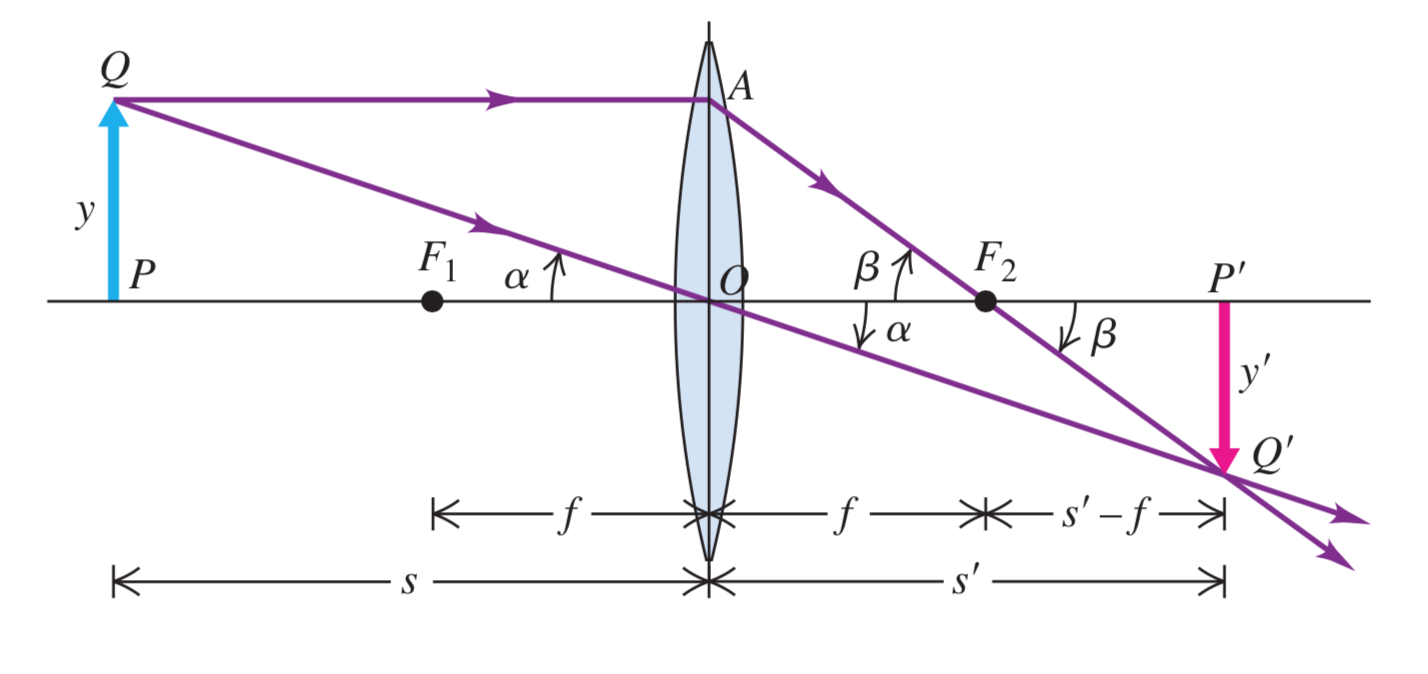
\includegraphics[width=0.6\textwidth]{pictures/lenteConcavo.png}
\end{figure}

\end{frame}

\begin{frame}{Most Common Imaging Process}
\begin{figure}

{  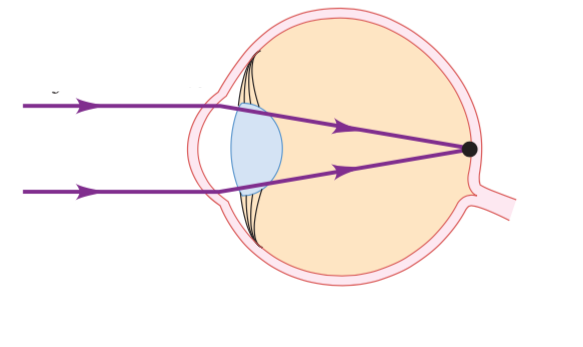
\includegraphics[width=0.4\textwidth]{pictures/ojoNormal.png} }
{  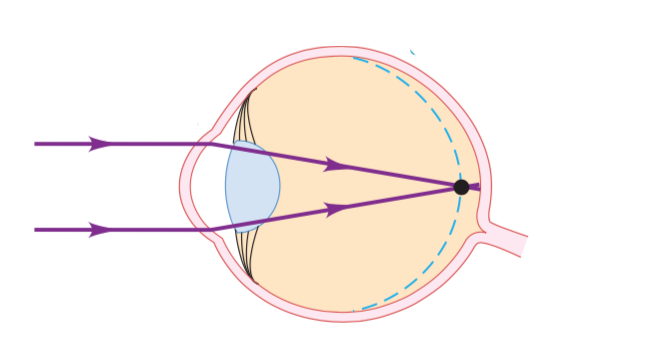
\includegraphics[width=0.4\textwidth]{pictures/ojoMiope.png} }
{  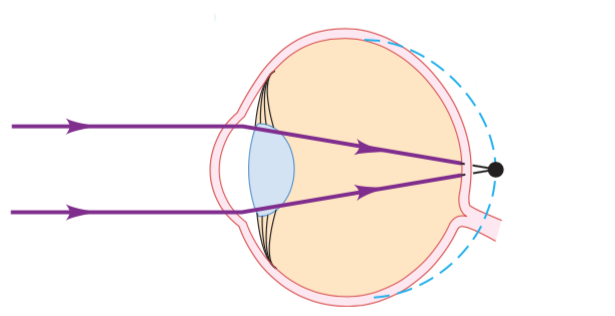
\includegraphics[width=0.4\textwidth]{pictures/ojoHipermetrope.png} }
\caption{Normal eye, Myopie and Hypermetropia}
 \label{n1}
 
\end{figure}
\end{frame}

\begin{frame}{Ghost Imaging Experimental Setup}
\begin{figure}
 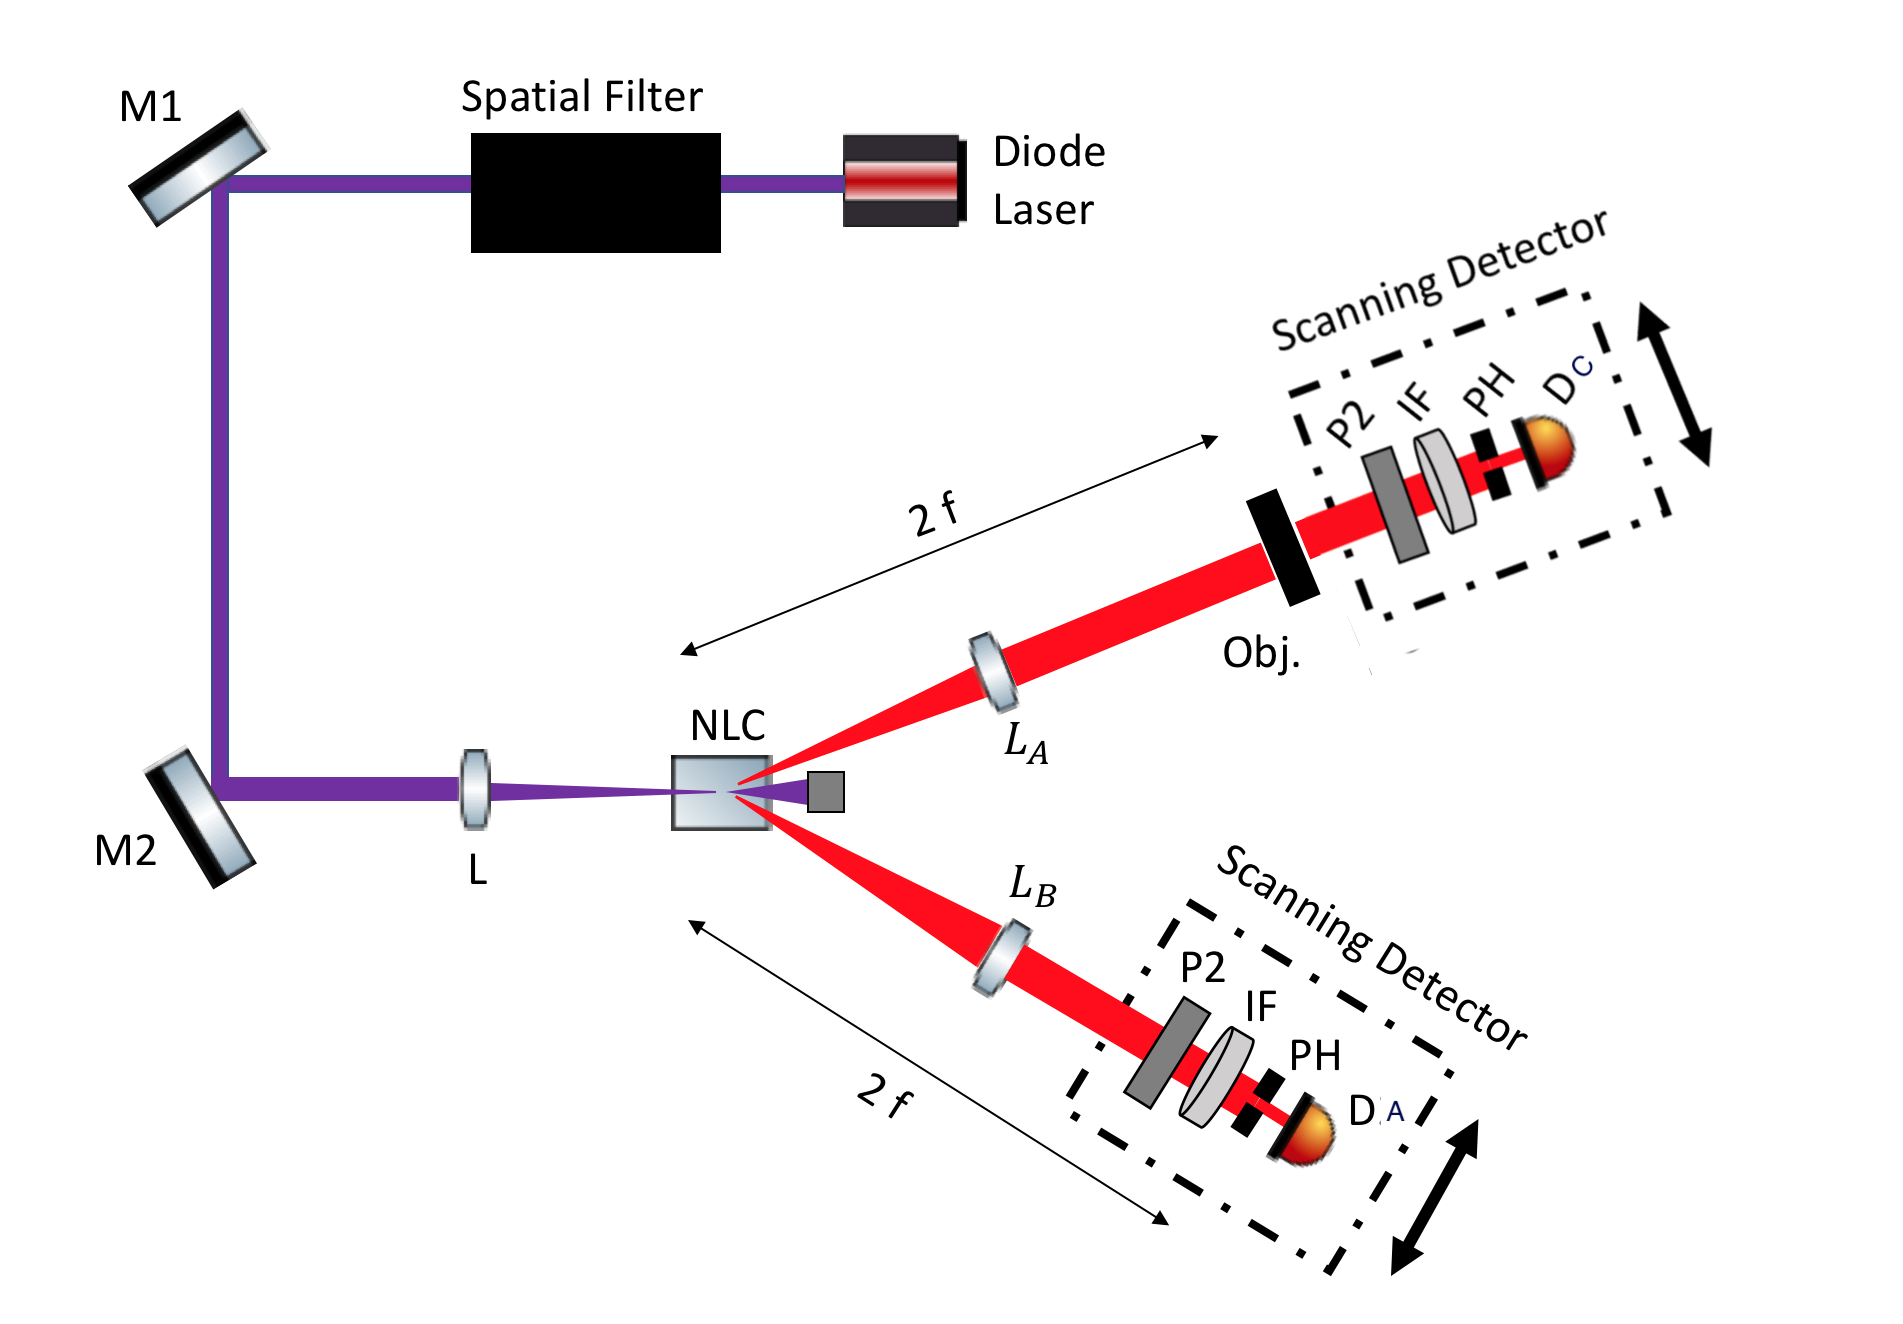
\includegraphics[width=0.6\textwidth]{pictures/setup.png}
 \caption{Experimental Setup for Alignment} 
 \end{figure}
\end{frame}

\begin{frame}{Ghost Imaging Experimental Setup}
\begin{figure}
 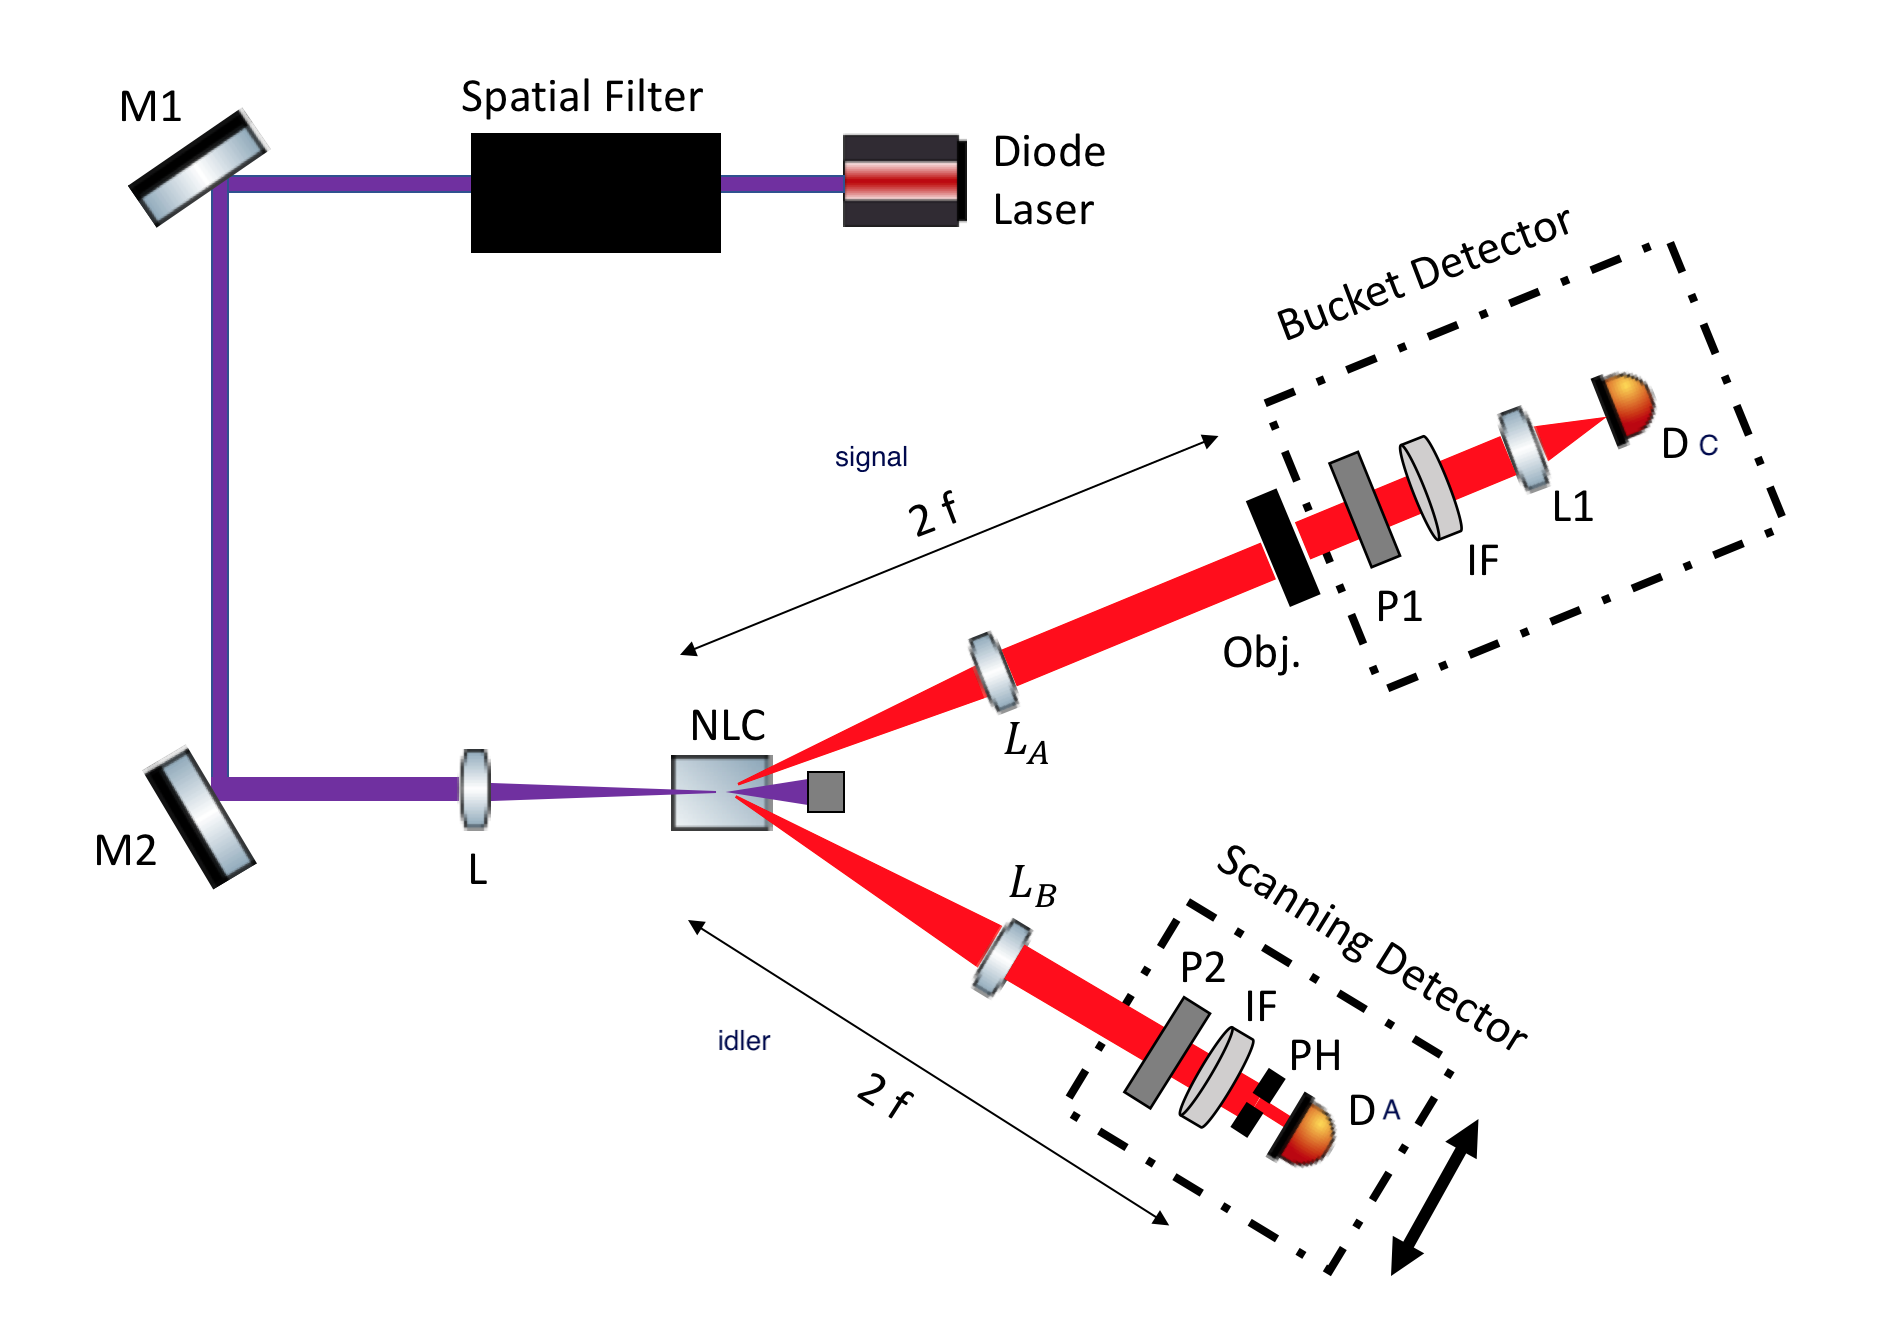
\includegraphics[width=0.6\textwidth]{pictures/setup2.png}
 \caption{Experimental Setup for Ghost Imaging} 
 \end{figure}
\end{frame}

\begin{frame}{Biphoton}
\begin{center}
\begin{equation}

\ket{\Psi}=\int{dq_s dq_i d\Omega_s d\Omega_i \\
x [\Phi(q_s,\Omega_s;q_i,\Omega_i) \hat{a}^{\dagger} (\Omega_s,q_s) \hat{a}^{\dagger}(\Omega_i,q_i) \\ + \Phi(q_i,\Omega_i;q_s,\Omega_s) \hat{a}^{\dagger}(\Omega_s,q_s) \hat{a}^{\dagger}(\Omega_i,q_i)]   \ket{0}} \\
\caption{}
\end{equation}
\end{center}
\item After using Polarisers this reduces to:
\begin{equation*}

\ket{\Psi}=\int{dq_s dq_i d\Omega_s d\Omega_i 
x [\Phi(q_s,\Omega_s;q_i,\Omega_i) \hat{a}^{\dagger} (\Omega_s,q_s) \hat{a}^{\dagger}(\Omega_i,q_i)] \ket{0}} \\
\caption{}
\end{equation*}

\end{frame}

\begin{frame}{Nonlinear Crystal (BBO)}
\begin{figure}

{  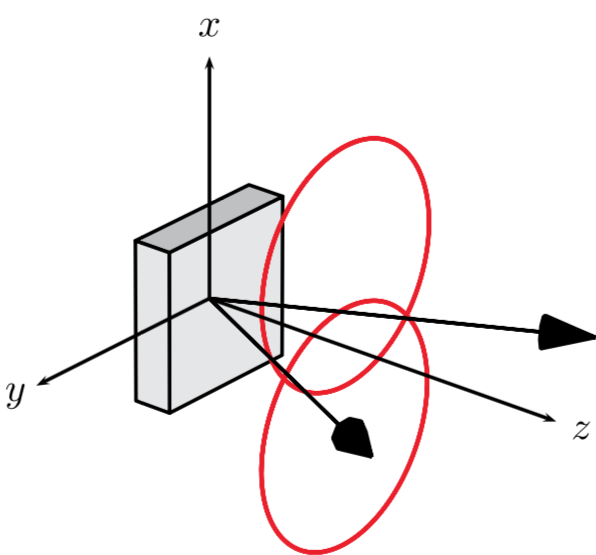
\includegraphics[width=0.3\textwidth]{pictures/BBO.png} }
{  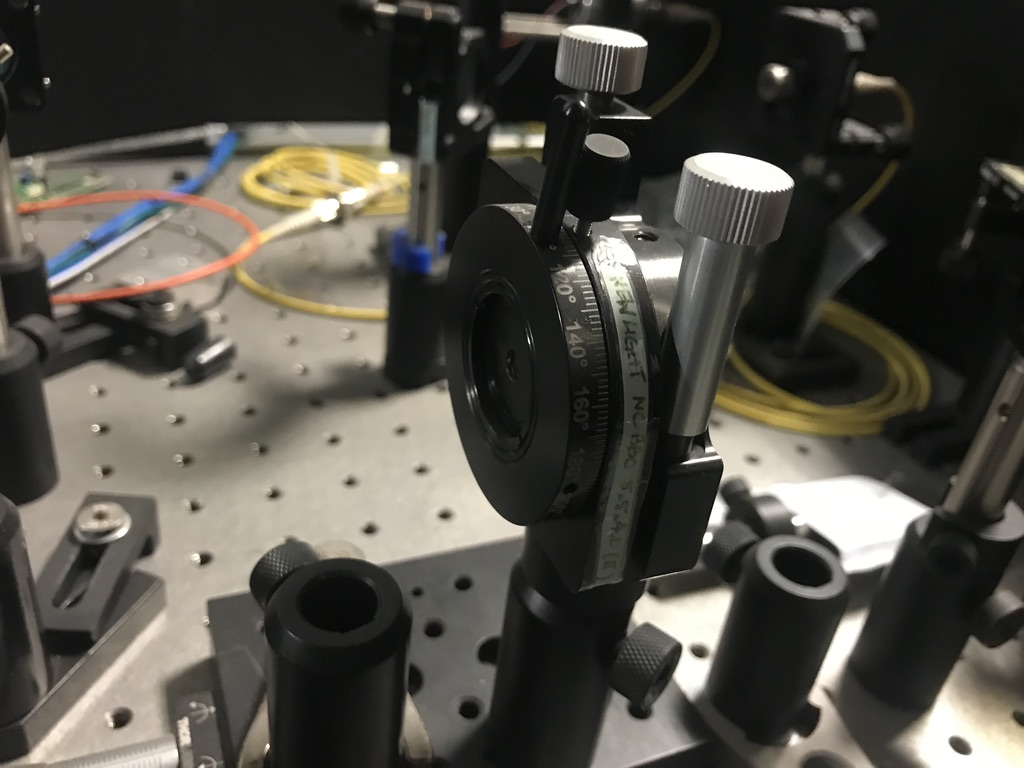
\includegraphics[width=0.4\textwidth]{pictures/BBOExp.jpg} }
{  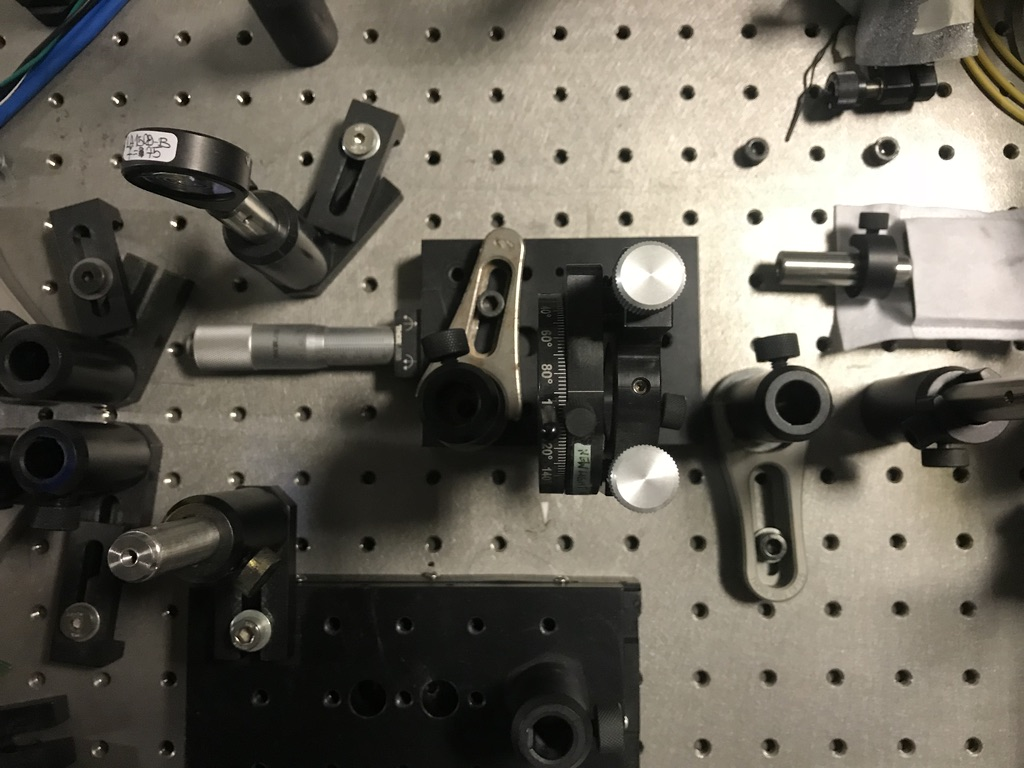
\includegraphics[width=0.4\textwidth]{pictures/BBOExp2.jpg} }
\caption{Normal eye, Myopie and Hypermetropia}
 \label{n1}
 
\end{figure}
\end{frame}

%\begin{frame}{Phase matching conditions}
%\begin{equation*}
%\Delta_0 = q^y_s cos \varphi_s + q^y_i cos \varphi_i + k_s sin \varphi_s - k_i sin \varphi_i ;
%\end{equation*}
%\begin{equation*}
%\Delta_k = k_p - k_s cos \varphi_s - k_i cos \varphi_i - q^y_s sin \varphi_s + q^y_i sin \varphi_i 
%\end{equation*}
%\begin{equation*}+ (q^x_s + q^x_i ) tan \rho_0 cos \alpha + \Delta_0 tan \rho_0 sin \alpha \end{equation*}


%\renewcommand\windowpagestuff{%
 % 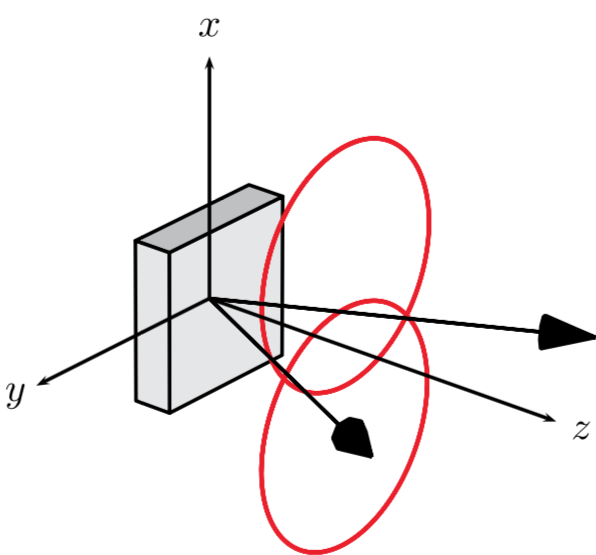
\includegraphics[height=2.5cm, width=1.5cm]{pictures/BBO.png}
  %\par{\usebeamercolor[fg]{caption name}%
  %\usebeamerfont*{caption name}\figurename%
  %\usebeamertemplate{caption label separator}}%
% \raggedright%
  %\usebeamerfont*{caption}%
  %captions no necesary.%
%}
%\opencutleft
%\vfill

%\begin{cutout}{0}{0pt}{.8\linewidth}{4}
%where $k_n=[(\omega^0_n n_n / c )^2 - |q_n|^2]^{\frac{1}{2}}$ is the longitudinal wavevector inside the crystal. $\varphi_s$ and $\varphi_i$ are the propagation directions of the generated photons inside the crystal with respect to the pump direction $z$ and $\alpha$ is the azimuthal angle.
%\end{cutout}
%\end{frame}


\begin{frame}{Tracing Out Temporal Correlations}


To Observe the transverse correlations the frequency information has to be traced out.
\renewcommand\windowpagestuff{%
  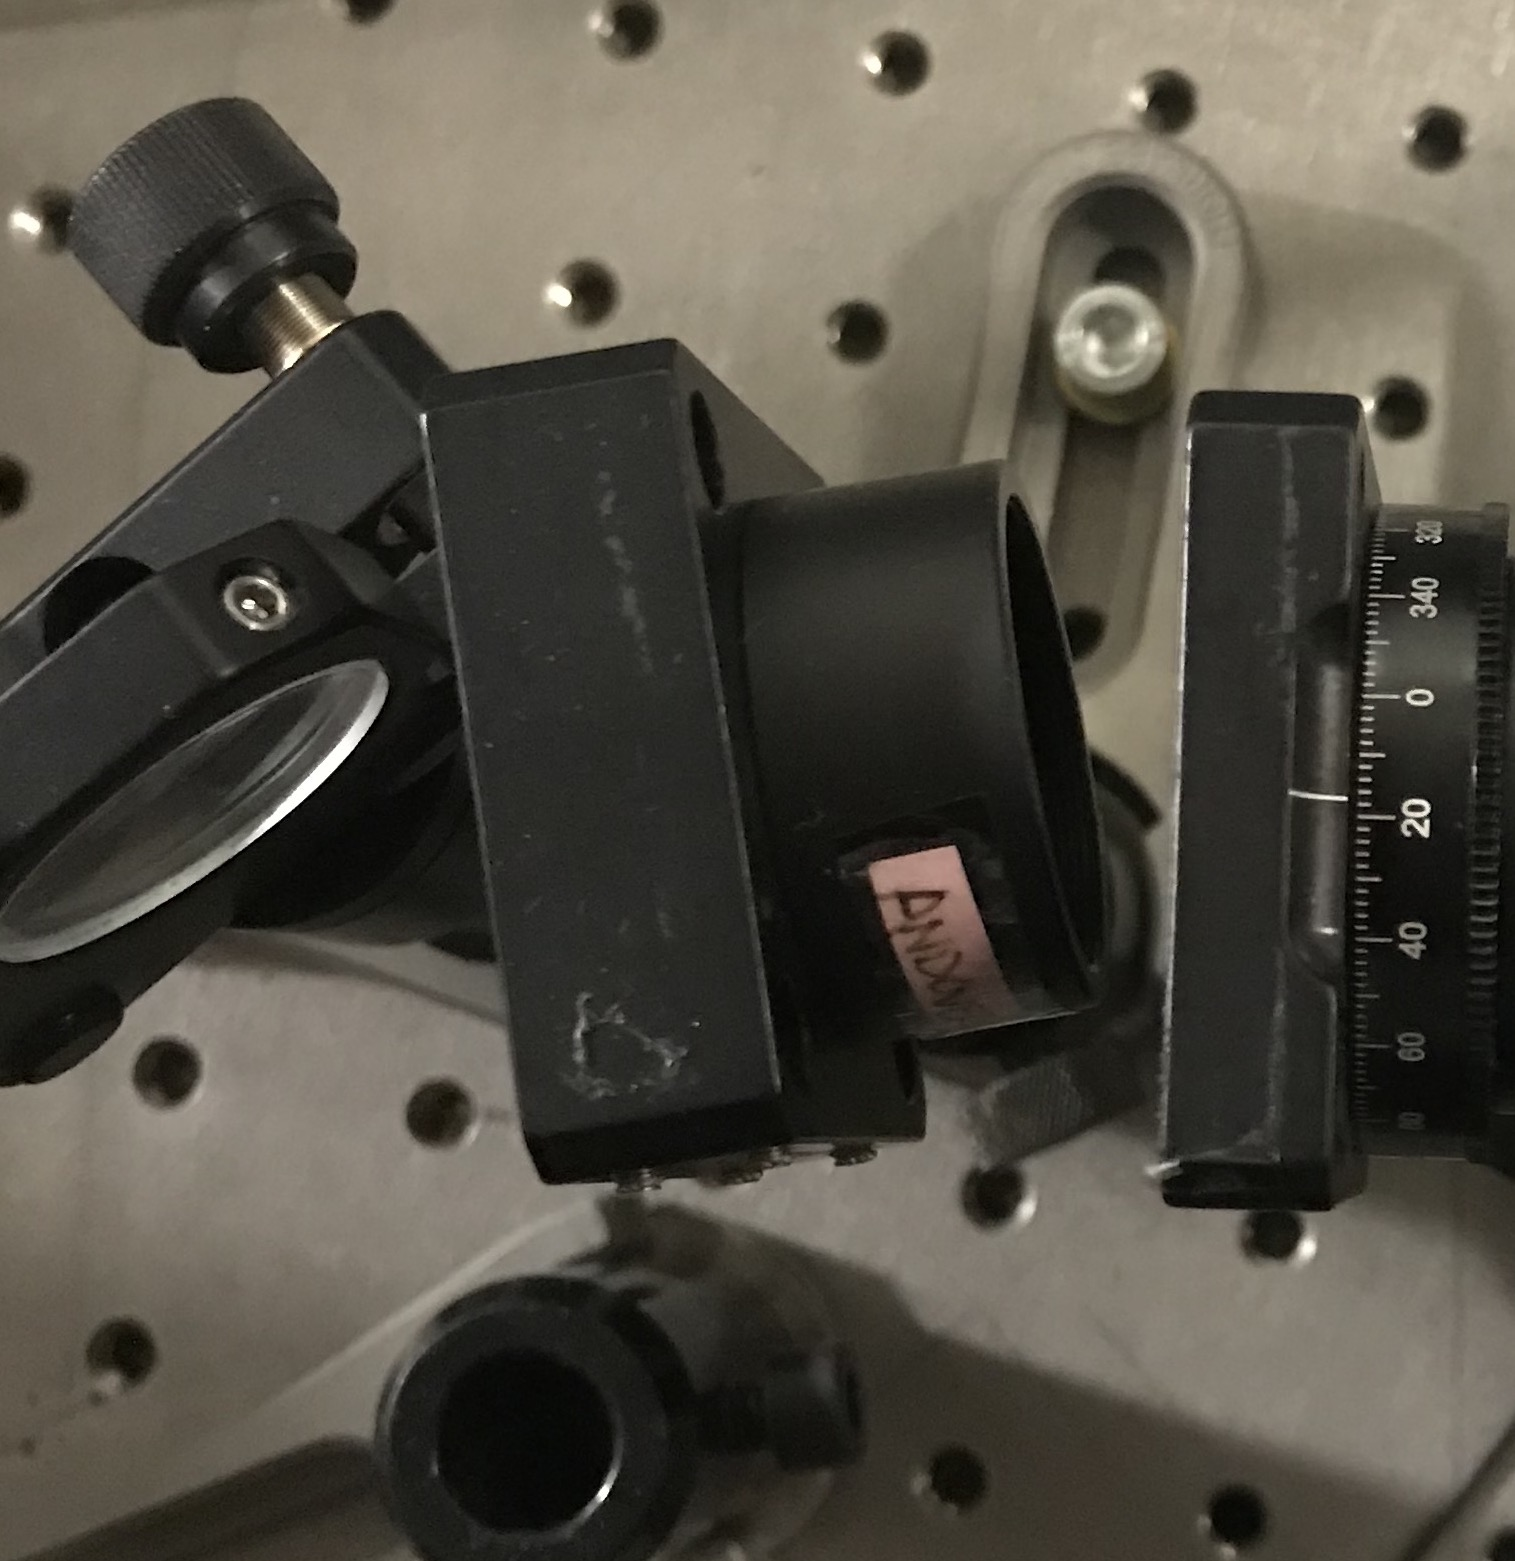
\includegraphics[height=2.5cm, width=2.5cm]{pictures/frequencyFilter.jpg}
  \raggedright
  
}
\opencutleft
\vfill

\begin{cutout}{0}{0pt}{0.75\linewidth}{4}
\begin{equation*}
\mathcal{F}_{frequency}(\Omega_n) \approx exp \left[-\frac{ \Omega^2_n}{4 \sigma^2_n} \right] 
\end{equation*}
\begin{equation*}
\tilde{\Phi}(q_s,q_i)=\int d\Omega_s d\Omega_i \mathcal{F}_s (\Omega_s) \mathcal{F}_i (\Omega_i) \Phi(q_s,\Omega_s;q_i,\Omega_i)
\end{equation*}
\end{cutout}
\end{frame}



\begin{frame}{Correlations Degree (DOC)}
A way to quantify the degree of spatial correlation we shall define 'correlation parameter':
\begin{equation*}
K^\lambda = \frac{C^\lambda_{si}}{\sqrt{C^\lambda_{ss}C^\lambda_{ii}}}
\end{equation*}
calculated for each direction $(\lambda = x, y)$ from the covariance matrix $C^\lambda$ with elements $C^\lambda_{kj} = \langle q^\lambda_k q^\lambda_j \rangle - \langle q^\lambda_k \rangle \langle q^\lambda_j \rangle $.
\end{frame}

\begin{frame}{DOC vs $w_p$}
\begin{figure}

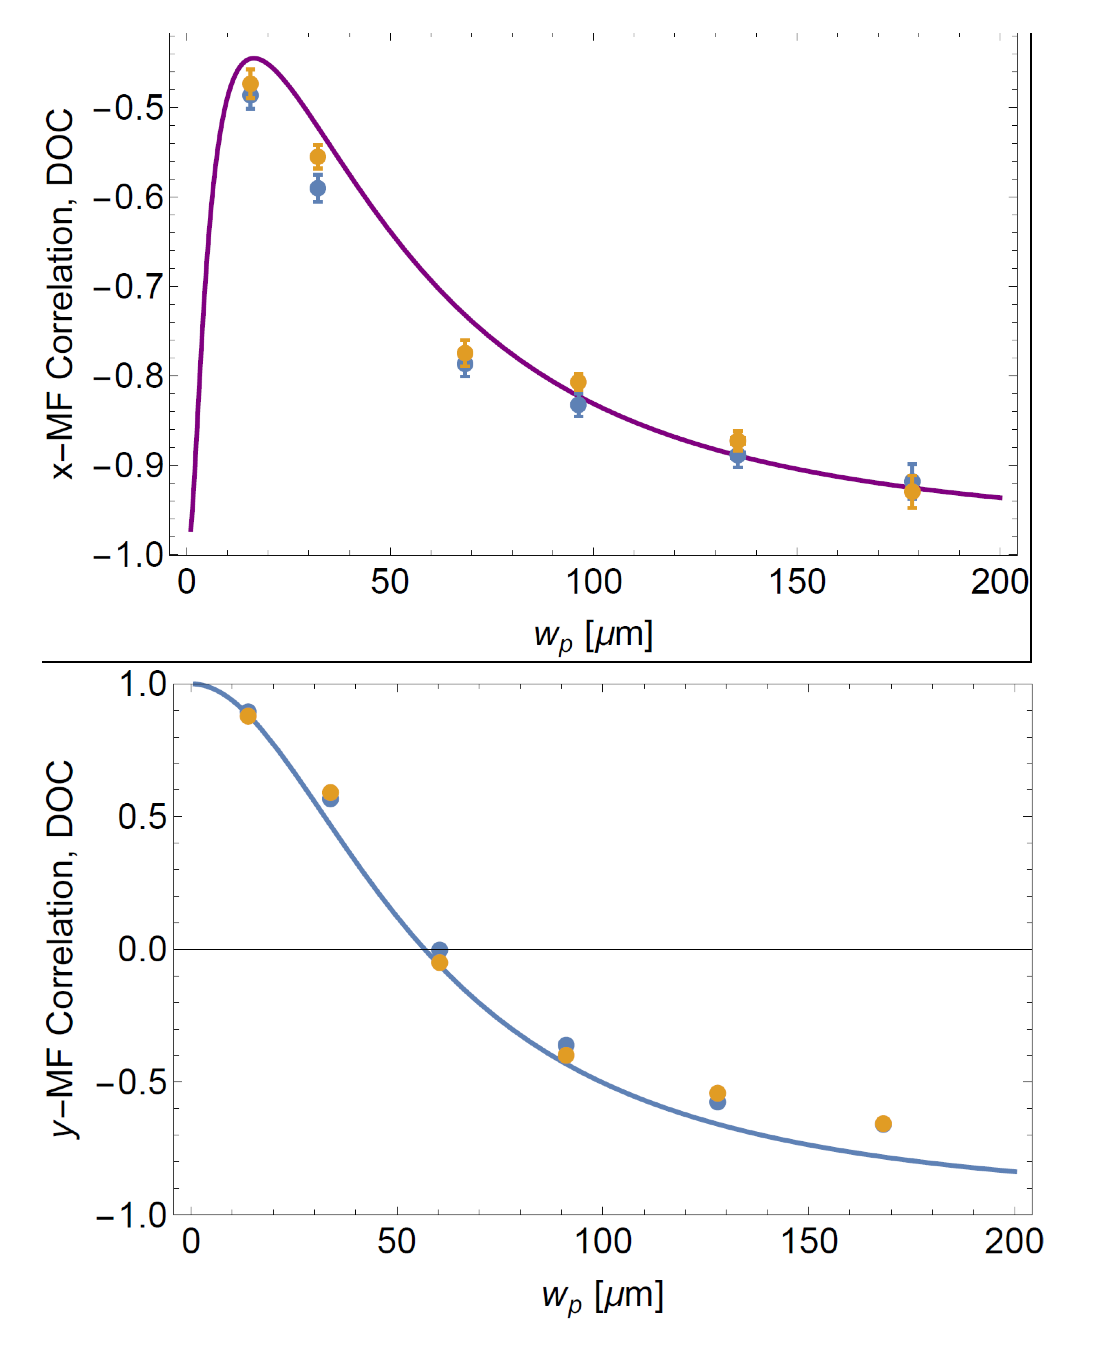
\includegraphics[width=0.5\textwidth]{pictures/correlationGraph.png} 

\caption{taken from \ref{omar}}
 \label{n1}
\end{figure}
\end{frame}
\begin{frame}{Fourier Plane}
\item Using Fourier one to one correspondence  between the transverse momentum and
position $q = \frac{2 \pi}{\lambda f} r$.
\begin{figure}

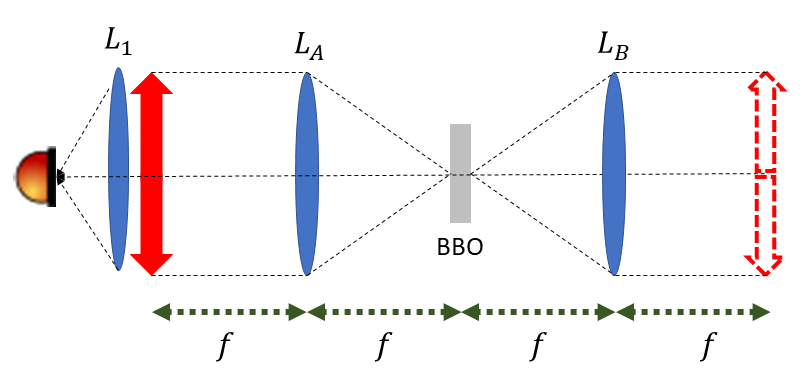
\includegraphics[width=0.5\textwidth]{pictures/2f.png} 

%\caption{taken from \ref{omar}}
 \label{n1}
\end{figure}
\end{frame}

\begin{frame}{Detection}

\item The coincidence counts that will be measured by the Detectors will be proportional to the magnitude square of the resulting biphoton function $\Phi_1 (r_2)$.
\begin{equation}
S(r_2) \propto |  \int d^2 r_1 T(r_1) \Phi (\frac{2 \pi}{\lambda f}r_1, \frac{2 \pi}{\lambda f}r_2) |^2
\end{equation}
\end{frame}
\begin{frame}{Numerical Example}
\begin{figure}

%{  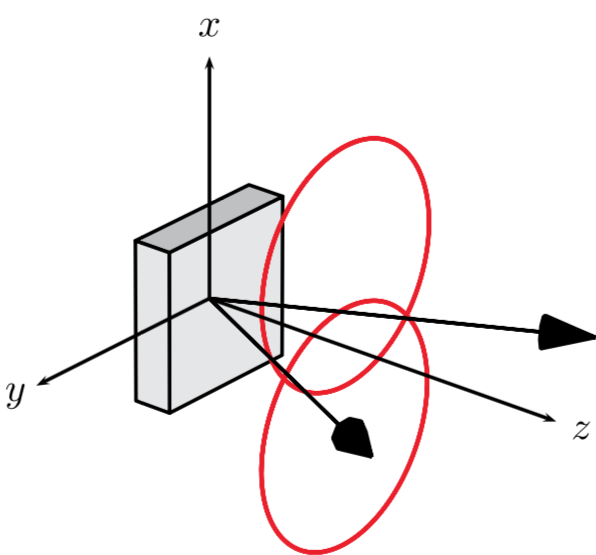
\includegraphics[width=0.3\textwidth]{pictures/BBO.png} }
{  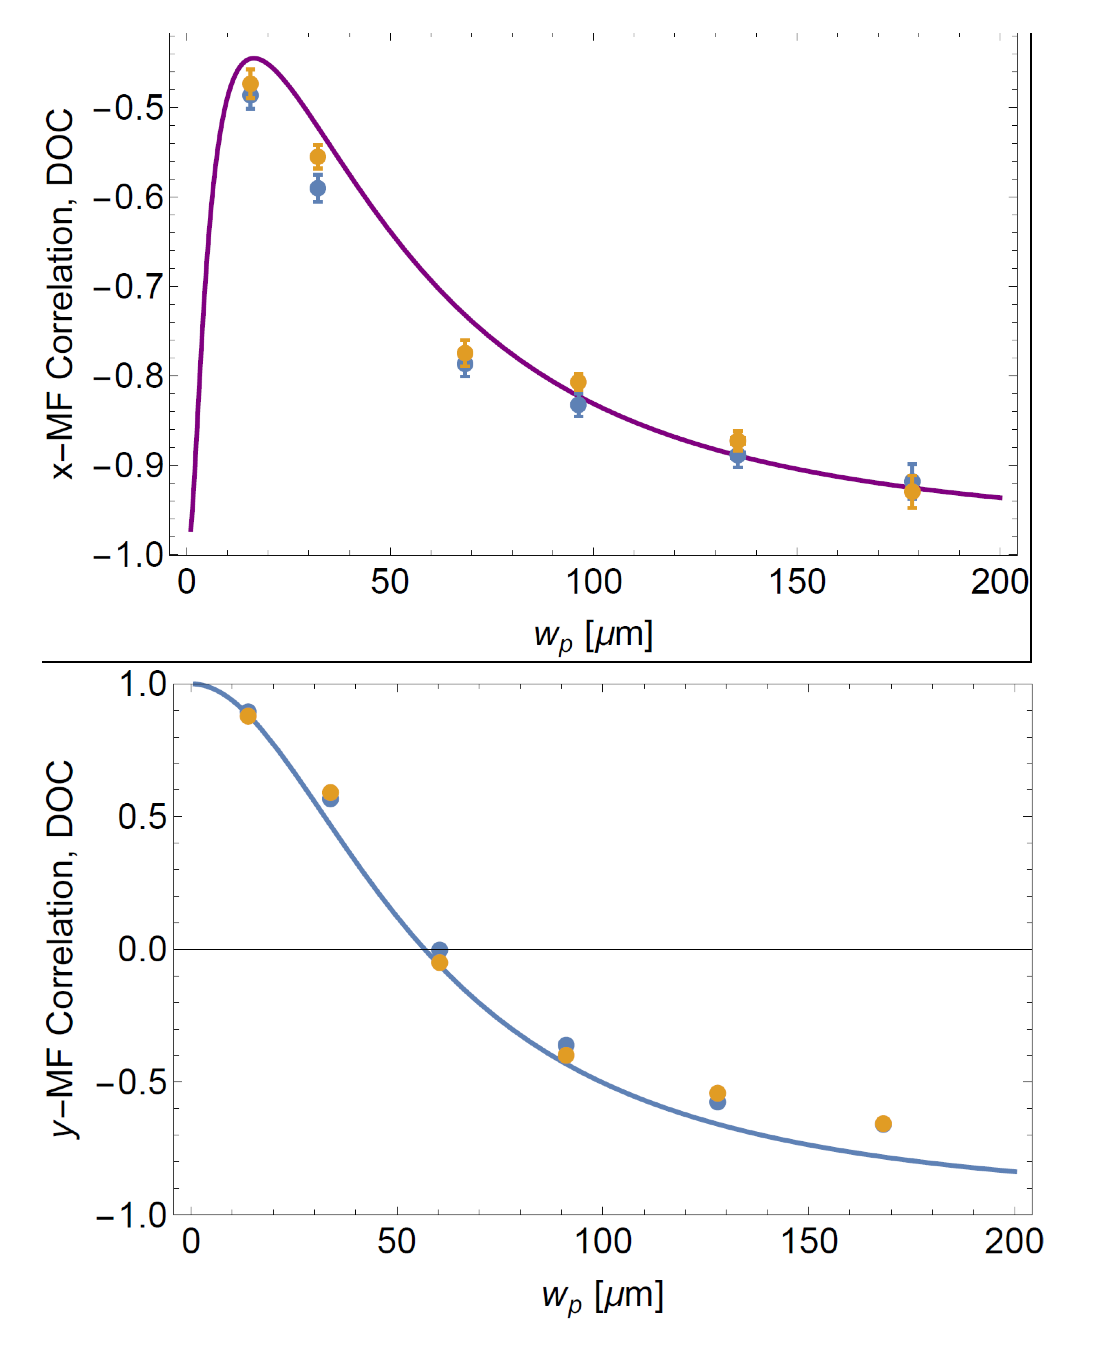
\includegraphics[width=0.4\textwidth]{pictures/correlationGraph.png} }
%{  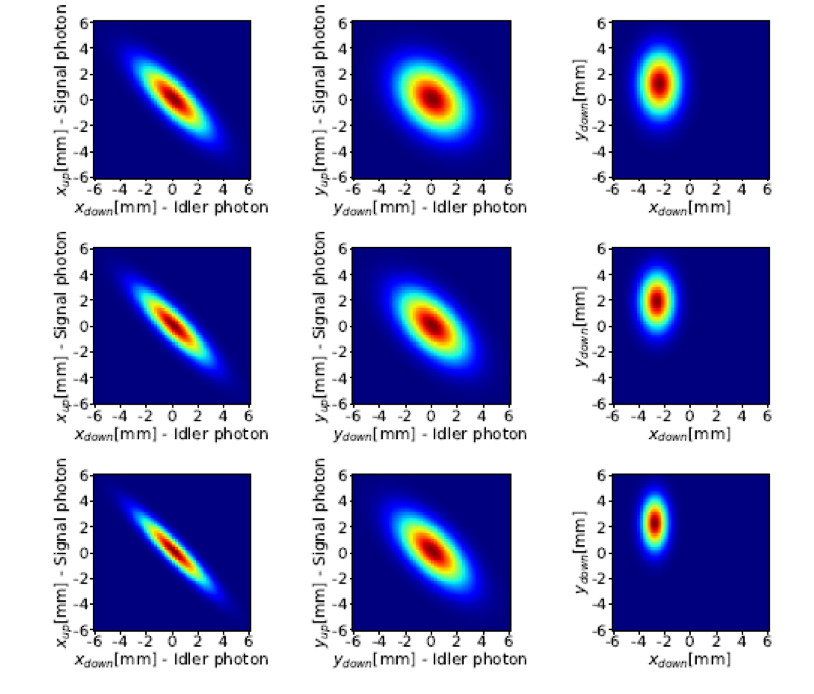
\includegraphics[width=0.45\textwidth]{pictures/correlaciones2.png} }
{  
\includegraphics[width=0.2\textwidth]{pictures/mask.png} }
\caption{Mask used}
 \label{n1}
 
\end{figure}

\end{frame}
\begin{frame}{Numerical Example}

\begin{figure}

%{  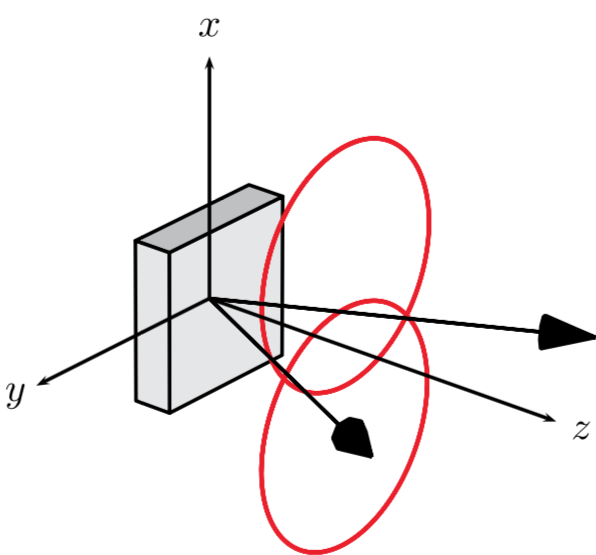
\includegraphics[width=0.3\textwidth]{pictures/BBO.png} }
{  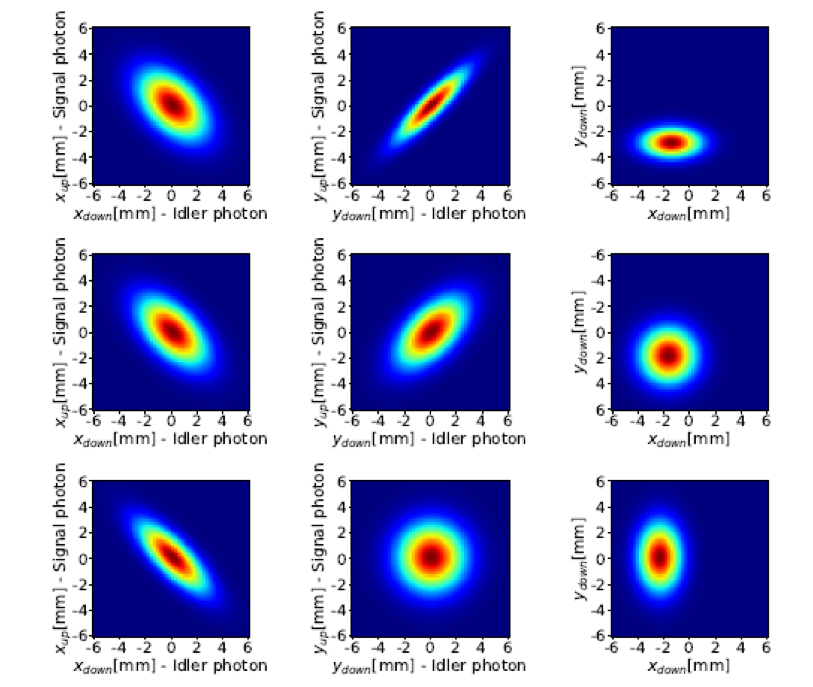
\includegraphics[width=0.45\textwidth]{pictures/correlaciones.png} }
{  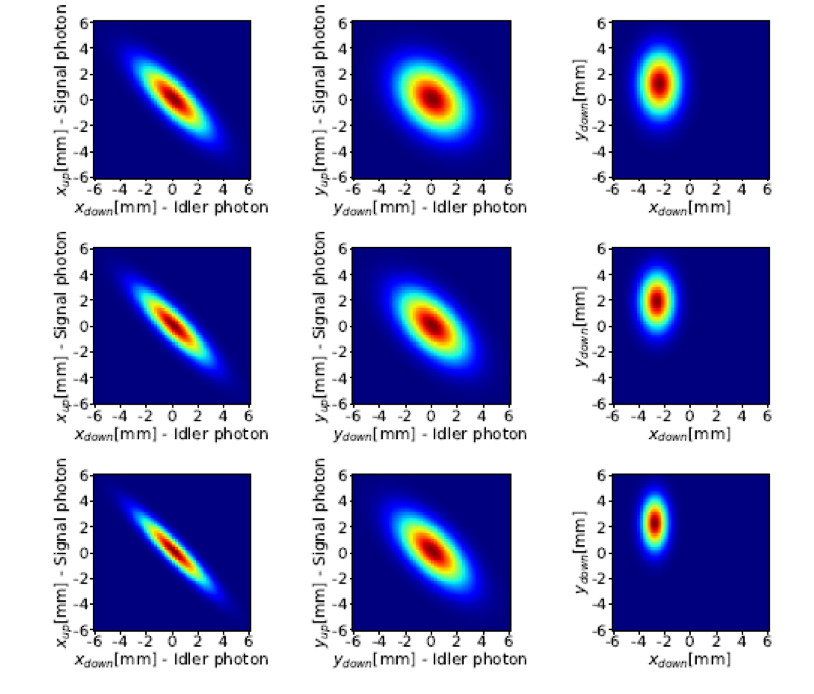
\includegraphics[width=0.45\textwidth]{pictures/correlaciones2.png} }
%\caption{Normal eye, Myopie and Hypermetropia}
 \label{n1}
 
\end{figure}
\end{frame}

\begin{frame}{Experiment at Uniandes: Results}

\begin{figure}
 \centering

{  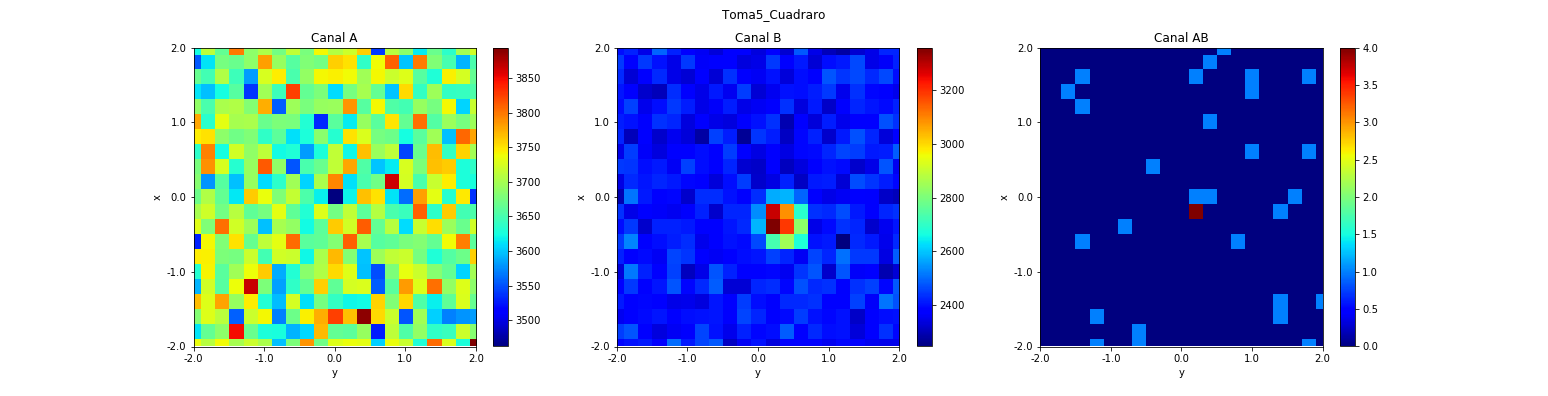
\includegraphics[width=0.9\textwidth]{pictures/Toma5_Cuadraro.png} }
{  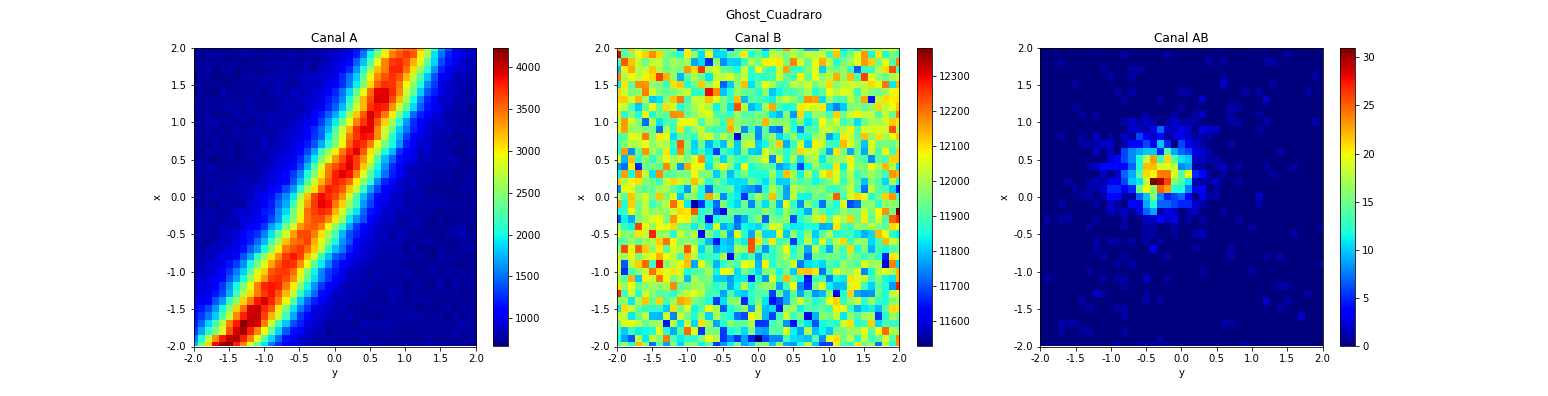
\includegraphics[width=0.9\textwidth]{pictures/Ghost_Cuadraro.png} }
\caption{Alignment and Ghost Image square 4x4 \mu m}
 \label{n1}
\end{figure}

\end{frame}

\begin{frame}
\begin{figure}
 \centering

{  
\includegraphics[width=0.4\textwidth]{pictures/interrogation.png} }
{  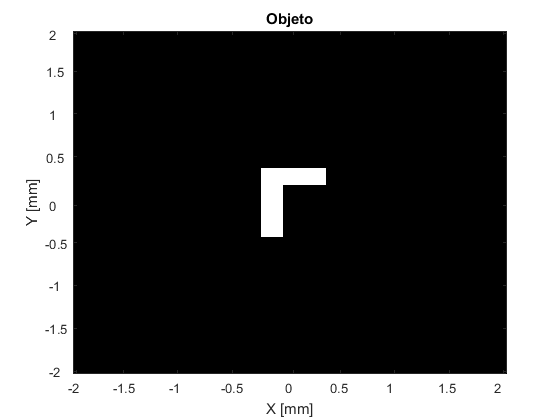
\includegraphics[width=0.4\textwidth]{pictures/L.png} }
\caption{Mask Used so far}
 \label{n1}
\end{figure}
\end{frame}

\begin{frame}
\begin{figure}
 \centering

{  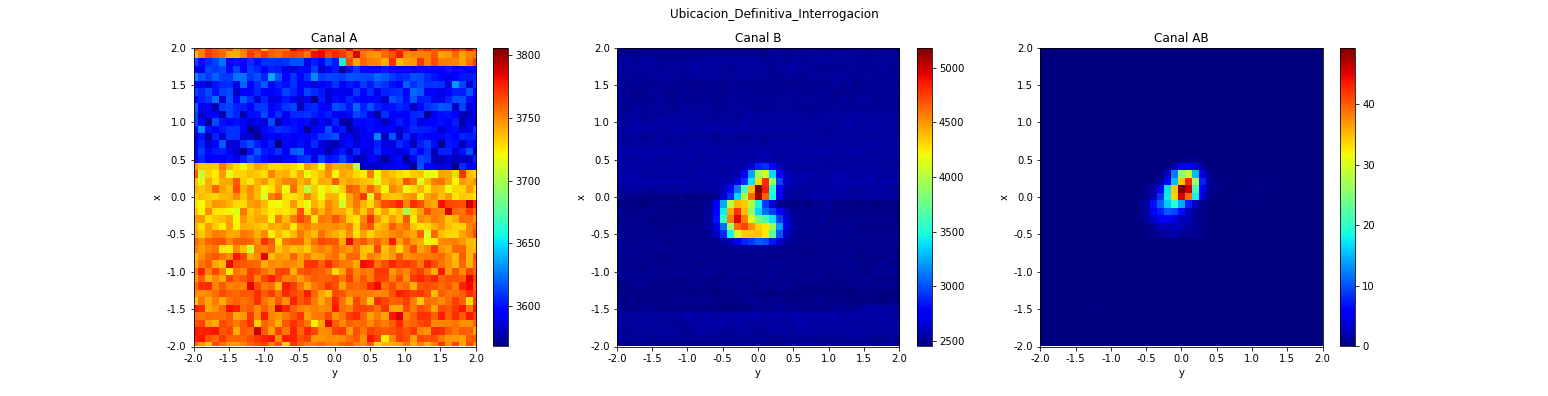
\includegraphics[width=0.9\textwidth]{pictures/Ubicacion_Definitiva_Interrogacion.png} }
{  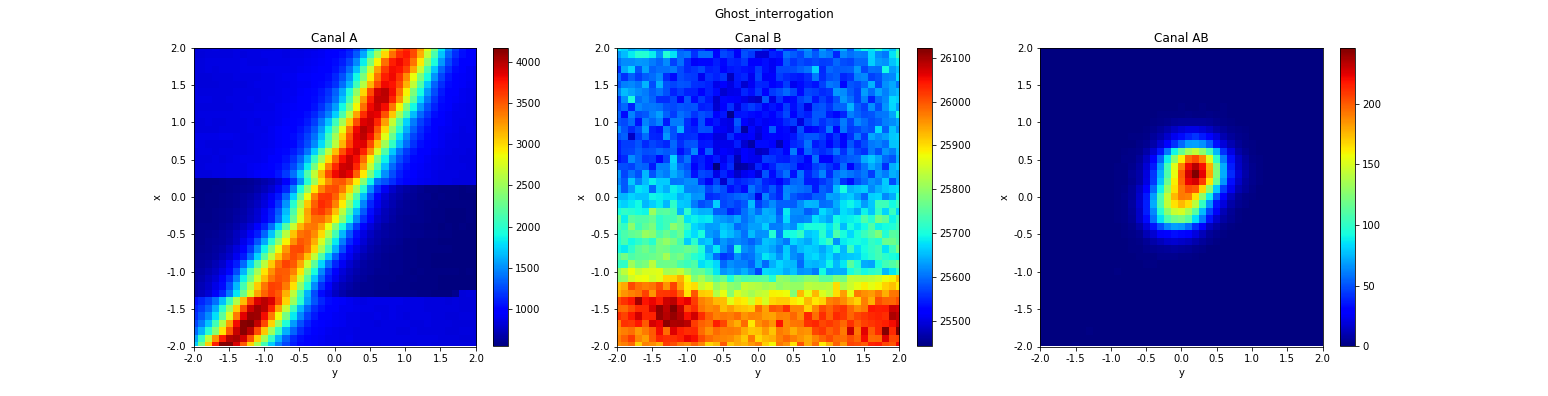
\includegraphics[width=0.9\textwidth]{pictures/Ghost_interrogation.png} }
\caption{Alignment and Ghost Image interrogation}
 \label{n1}
\end{figure}
\end{frame}


\begin{frame}
\begin{figure}
 \centering

{  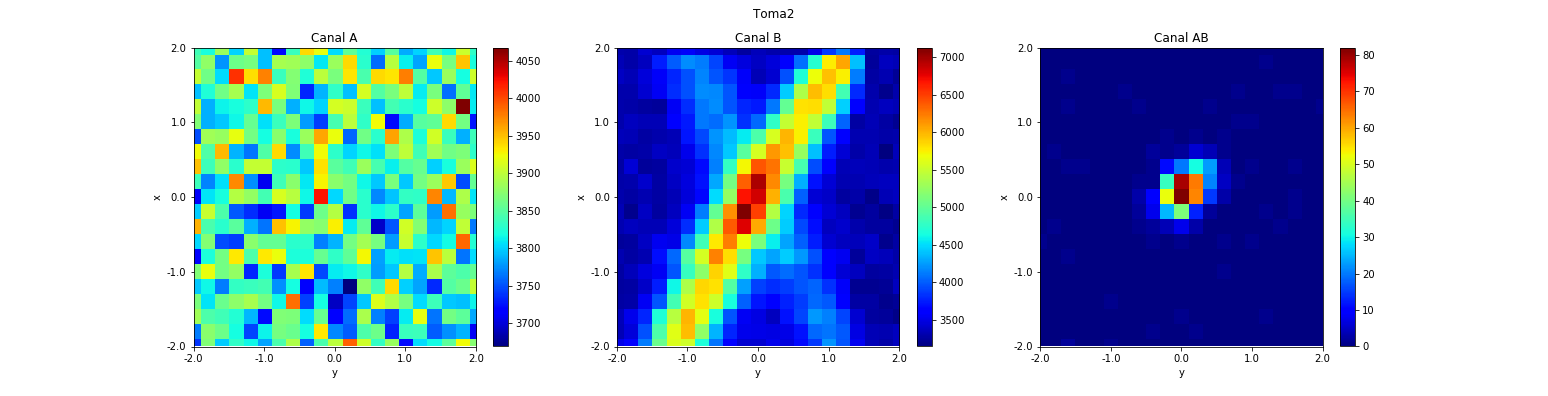
\includegraphics[width=0.9\textwidth]{pictures/Toma2.png} }
{  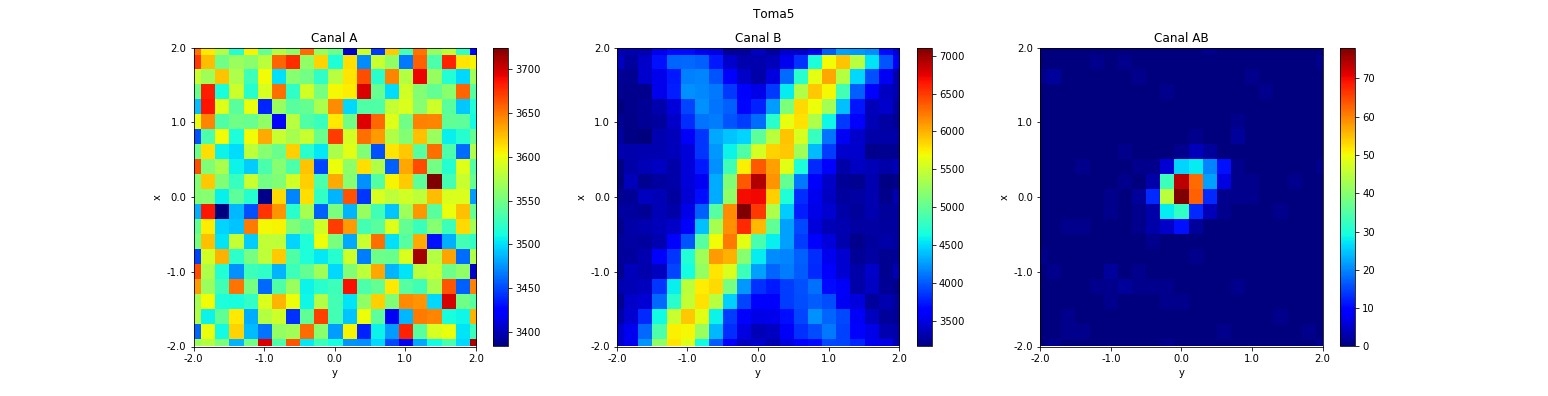
\includegraphics[width=0.9\textwidth]{pictures/Toma5.png} }
\caption{Alignment for the L}
 \label{n1}
\end{figure}
\end{frame}

\begin{frame}
\begin{figure}
 \centering

{  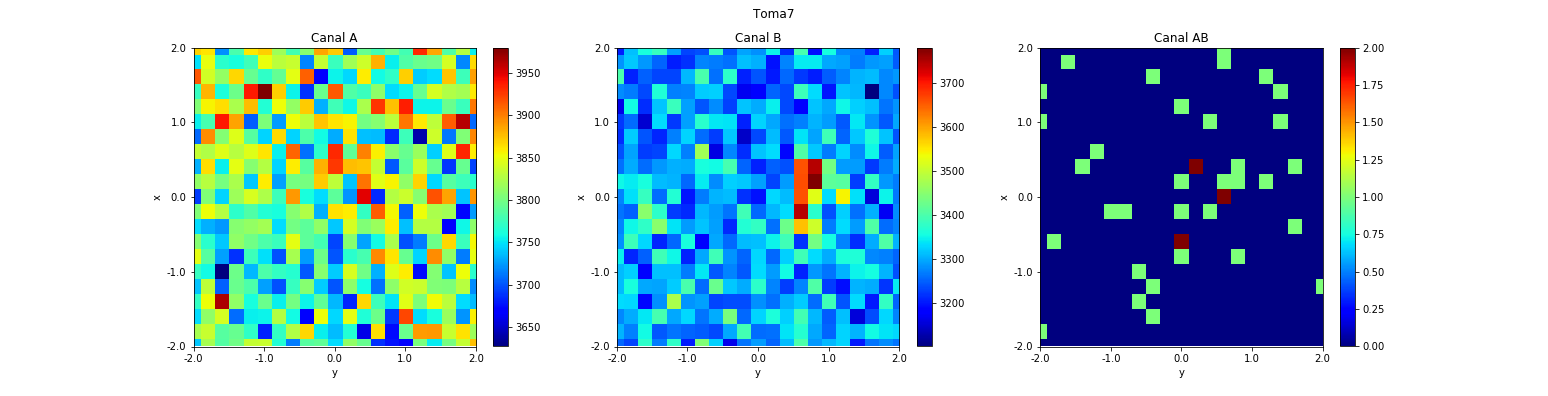
\includegraphics[width=0.9\textwidth]{pictures/Toma7.png} }
{  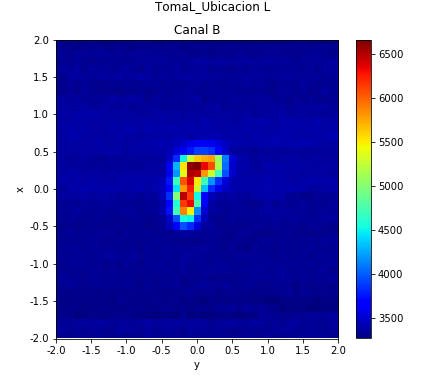
\includegraphics[width=0.9\textwidth]{pictures/TomaL_UbicacionL.png} }
\caption{Alignment for the L}
 \label{n1}
\end{figure}
\end{frame}

\begin{frame}
\begin{figure}
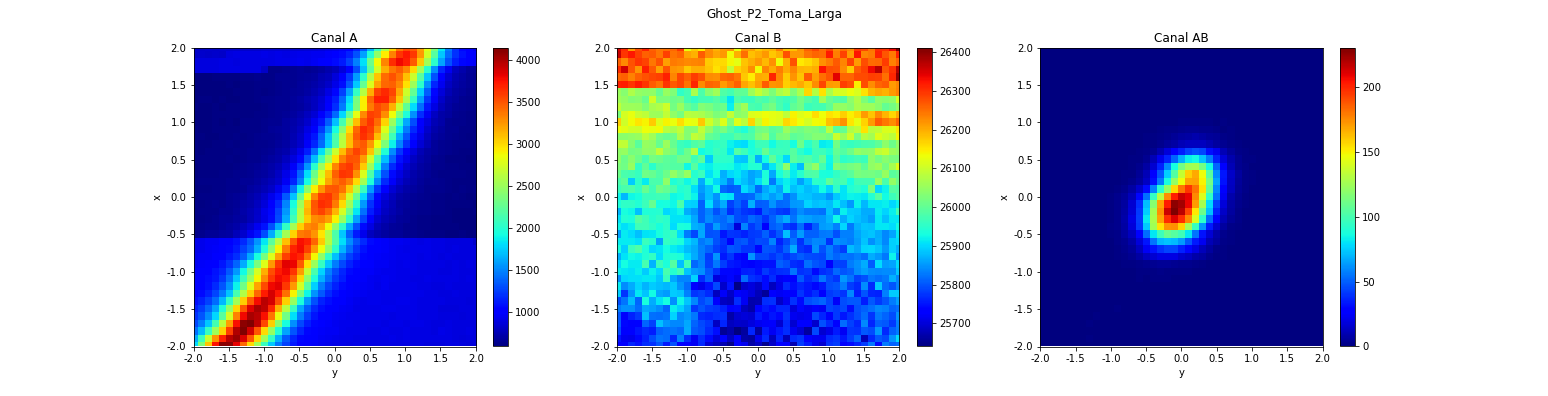
\includegraphics[width=1.1\textwidth]{pictures/Ghost_P2_Toma_Larga.png}
\caption{Ghost Long Measurement}
\end{figure}
\end{frame}
\begin{frame}{Experimental vs. Simulation Results}
\begin{figure}
 \centering

{  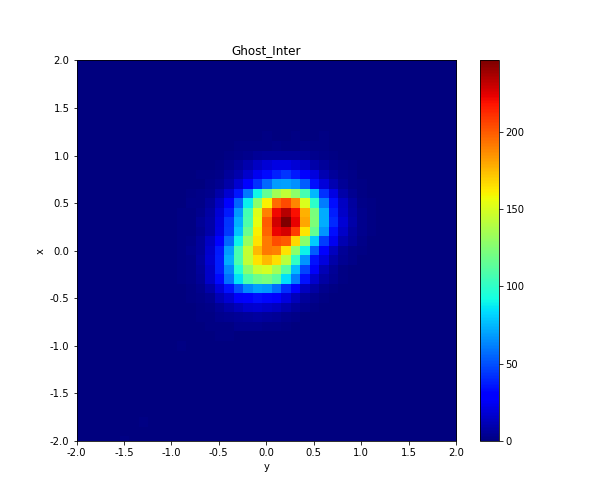
\includegraphics[width=0.4\textwidth]{pictures/Ghost_Inter.png} }
{  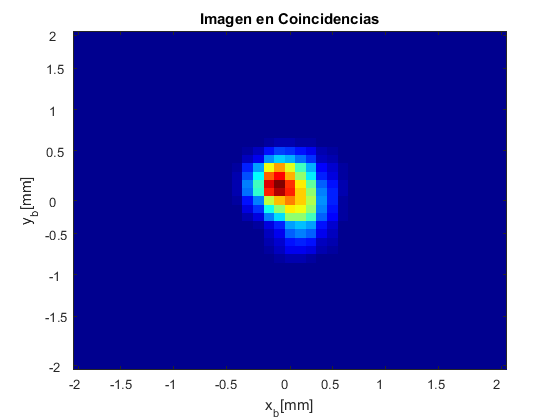
\includegraphics[width=0.4\textwidth]{pictures/ImagenS1.png} }
\caption{Comparison for the Interrrogation}
 \label{n1}
\end{figure}
\end{frame}
\begin{frame}
\begin{figure}
 \centering

{  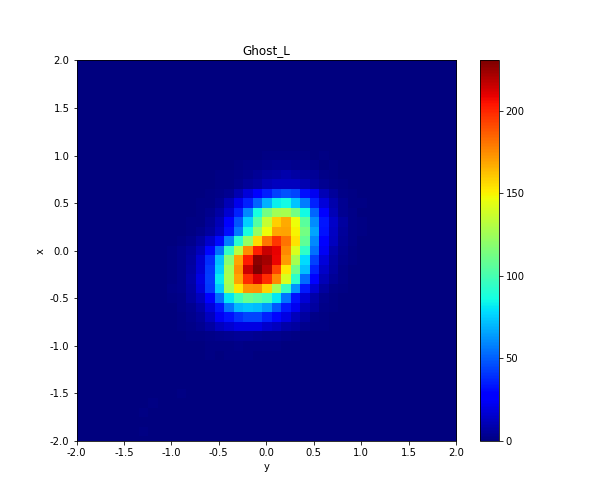
\includegraphics[width=0.4\textwidth]{pictures/Ghost_L.png} }
{  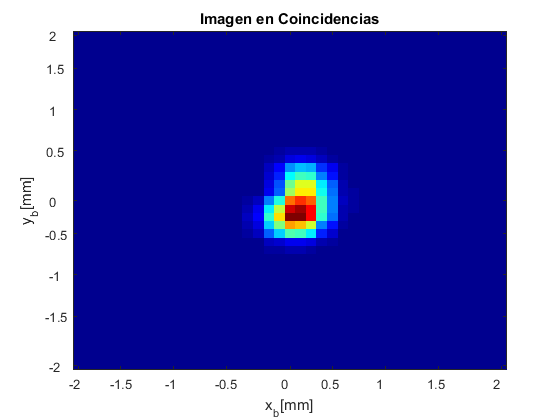
\includegraphics[width=0.4\textwidth]{pictures/Imagen_41x41.png} }
\caption{Comparison for the L}
 \label{n1}
\end{figure}

\end{frame}




\begin{frame}{Bibliography}
\bibliographystyle{plainnat}
\bibliography{bibli.bib}
\end{frame}









    
  


\end{document}


